% Options for packages loaded elsewhere
\PassOptionsToPackage{unicode}{hyperref}
\PassOptionsToPackage{hyphens}{url}
\PassOptionsToPackage{dvipsnames,svgnames,x11names}{xcolor}
%
\documentclass[
]{article}

\usepackage{amsmath,amssymb}
\usepackage{lmodern}
\usepackage{iftex}
\ifPDFTeX
  \usepackage[T1]{fontenc}
  \usepackage[utf8]{inputenc}
  \usepackage{textcomp} % provide euro and other symbols
\else % if luatex or xetex
  \usepackage{unicode-math}
  \defaultfontfeatures{Scale=MatchLowercase}
  \defaultfontfeatures[\rmfamily]{Ligatures=TeX,Scale=1}
\fi
% Use upquote if available, for straight quotes in verbatim environments
\IfFileExists{upquote.sty}{\usepackage{upquote}}{}
\IfFileExists{microtype.sty}{% use microtype if available
  \usepackage[]{microtype}
  \UseMicrotypeSet[protrusion]{basicmath} % disable protrusion for tt fonts
}{}
\makeatletter
\@ifundefined{KOMAClassName}{% if non-KOMA class
  \IfFileExists{parskip.sty}{%
    \usepackage{parskip}
  }{% else
    \setlength{\parindent}{0pt}
    \setlength{\parskip}{6pt plus 2pt minus 1pt}}
}{% if KOMA class
  \KOMAoptions{parskip=half}}
\makeatother
\usepackage{xcolor}
\usepackage[margin = 1in]{geometry}
\setlength{\emergencystretch}{3em} % prevent overfull lines
\setcounter{secnumdepth}{5}
% Make \paragraph and \subparagraph free-standing
\ifx\paragraph\undefined\else
  \let\oldparagraph\paragraph
  \renewcommand{\paragraph}[1]{\oldparagraph{#1}\mbox{}}
\fi
\ifx\subparagraph\undefined\else
  \let\oldsubparagraph\subparagraph
  \renewcommand{\subparagraph}[1]{\oldsubparagraph{#1}\mbox{}}
\fi


\providecommand{\tightlist}{%
  \setlength{\itemsep}{0pt}\setlength{\parskip}{0pt}}\usepackage{longtable,booktabs,array}
\usepackage{calc} % for calculating minipage widths
% Correct order of tables after \paragraph or \subparagraph
\usepackage{etoolbox}
\makeatletter
\patchcmd\longtable{\par}{\if@noskipsec\mbox{}\fi\par}{}{}
\makeatother
% Allow footnotes in longtable head/foot
\IfFileExists{footnotehyper.sty}{\usepackage{footnotehyper}}{\usepackage{footnote}}
\makesavenoteenv{longtable}
\usepackage{graphicx}
\makeatletter
\def\maxwidth{\ifdim\Gin@nat@width>\linewidth\linewidth\else\Gin@nat@width\fi}
\def\maxheight{\ifdim\Gin@nat@height>\textheight\textheight\else\Gin@nat@height\fi}
\makeatother
% Scale images if necessary, so that they will not overflow the page
% margins by default, and it is still possible to overwrite the defaults
% using explicit options in \includegraphics[width, height, ...]{}
\setkeys{Gin}{width=\maxwidth,height=\maxheight,keepaspectratio}
% Set default figure placement to htbp
\makeatletter
\def\fps@figure{htbp}
\makeatother
\newlength{\cslhangindent}
\setlength{\cslhangindent}{1.5em}
\newlength{\csllabelwidth}
\setlength{\csllabelwidth}{3em}
\newlength{\cslentryspacingunit} % times entry-spacing
\setlength{\cslentryspacingunit}{\parskip}
\newenvironment{CSLReferences}[2] % #1 hanging-ident, #2 entry spacing
 {% don't indent paragraphs
  \setlength{\parindent}{0pt}
  % turn on hanging indent if param 1 is 1
  \ifodd #1
  \let\oldpar\par
  \def\par{\hangindent=\cslhangindent\oldpar}
  \fi
  % set entry spacing
  \setlength{\parskip}{#2\cslentryspacingunit}
 }%
 {}
\usepackage{calc}
\newcommand{\CSLBlock}[1]{#1\hfill\break}
\newcommand{\CSLLeftMargin}[1]{\parbox[t]{\csllabelwidth}{#1}}
\newcommand{\CSLRightInline}[1]{\parbox[t]{\linewidth - \csllabelwidth}{#1}\break}
\newcommand{\CSLIndent}[1]{\hspace{\cslhangindent}#1}

\usepackage{booktabs}
\usepackage{longtable}
\usepackage{array}
\usepackage{multirow}
\usepackage{wrapfig}
\usepackage{float}
\usepackage{colortbl}
\usepackage{pdflscape}
\usepackage{tabu}
\usepackage{threeparttable}
\usepackage{threeparttablex}
\usepackage[normalem]{ulem}
\usepackage{makecell}
\usepackage{xcolor}
\makeatletter
\makeatother
\makeatletter
\makeatother
\makeatletter
\@ifpackageloaded{caption}{}{\usepackage{caption}}
\AtBeginDocument{%
\ifdefined\contentsname
  \renewcommand*\contentsname{Table of contents}
\else
  \newcommand\contentsname{Table of contents}
\fi
\ifdefined\listfigurename
  \renewcommand*\listfigurename{List of Figures}
\else
  \newcommand\listfigurename{List of Figures}
\fi
\ifdefined\listtablename
  \renewcommand*\listtablename{List of Tables}
\else
  \newcommand\listtablename{List of Tables}
\fi
\ifdefined\figurename
  \renewcommand*\figurename{Figure}
\else
  \newcommand\figurename{Figure}
\fi
\ifdefined\tablename
  \renewcommand*\tablename{Table}
\else
  \newcommand\tablename{Table}
\fi
}
\@ifpackageloaded{float}{}{\usepackage{float}}
\floatstyle{ruled}
\@ifundefined{c@chapter}{\newfloat{codelisting}{h}{lop}}{\newfloat{codelisting}{h}{lop}[chapter]}
\floatname{codelisting}{Listing}
\newcommand*\listoflistings{\listof{codelisting}{List of Listings}}
\makeatother
\makeatletter
\@ifpackageloaded{caption}{}{\usepackage{caption}}
\@ifpackageloaded{subcaption}{}{\usepackage{subcaption}}
\makeatother
\makeatletter
\@ifpackageloaded{tcolorbox}{}{\usepackage[many]{tcolorbox}}
\makeatother
\makeatletter
\@ifundefined{shadecolor}{\definecolor{shadecolor}{rgb}{.97, .97, .97}}
\makeatother
\makeatletter
\makeatother
\ifLuaTeX
  \usepackage{selnolig}  % disable illegal ligatures
\fi
\IfFileExists{bookmark.sty}{\usepackage{bookmark}}{\usepackage{hyperref}}
\IfFileExists{xurl.sty}{\usepackage{xurl}}{} % add URL line breaks if available
\urlstyle{same} % disable monospaced font for URLs
\hypersetup{
  pdftitle={Younger, Unmarried, Childless, and Less Happy Americans Use the Internet the Most},
  pdfauthor={Sakura Ariga; Aliyah Maxine Ramos; Annie Yan},
  colorlinks=true,
  linkcolor={blue},
  filecolor={Maroon},
  citecolor={Blue},
  urlcolor={Blue},
  pdfcreator={LaTeX via pandoc}}

\title{Younger, Unmarried, Childless, and Less Happy Americans Use the
Internet the Most\thanks{Code and data are available at:
https://github.com/AnnieYan0807/GSS-data-analysis.git.}}
\usepackage{etoolbox}
\makeatletter
\providecommand{\subtitle}[1]{% add subtitle to \maketitle
  \apptocmd{\@title}{\par {\large #1 \par}}{}{}
}
\makeatother
\subtitle{An Analysis of the 2016 US General Social Survey}
\author{Sakura Ariga \and Aliyah Maxine Ramos \and Annie Yan}
\date{15 March 2023}

\begin{document}
\maketitle
\begin{abstract}
In this study, we investigated the 2016 United States General Social
Survey to gain an understanding of the characteristics of the people
that use the Internet the most, such as age, marital status, number of
children, and level of happiness. We did this by comparing the average
number of weekly Internet use across population groups. We found that
young adults that have never been married or have children and who are
not satisfied with their general happiness are those that use the
Internet the most. In an era in which the Internet is becoming more and
more used in the US, it is important to understand which population
group uses the Internet the most in order to inform public policies
surrounding Internet addiction and mental health.
\end{abstract}
\ifdefined\Shaded\renewenvironment{Shaded}{\begin{tcolorbox}[sharp corners, breakable, interior hidden, borderline west={3pt}{0pt}{shadecolor}, enhanced, frame hidden, boxrule=0pt]}{\end{tcolorbox}}\fi

\hypertarget{introduction}{%
\section{Introduction}\label{introduction}}

The Internet has become a widely used computer network that allows for
connection, communication, and access to information. By the mid 1990s,
the Internet began reaching millions of users from around the world,
where using a web of information, known as the World Wide Web, was a
popular way of browsing information and facilitating communication
online ({``A Short History of the Internet''} 2020). Throughout the
years, the different ways in which the Internet is used have expanded,
and now users can also make purchases through electronic commerce
platforms and share different forms of media on social media platforms.

This report aims to investigate the characteristics of American adults
that use the Internet the most in comparison to those that use it the
least. We aim to understand the reasons why these factors are correlated
with a higher Internet use pattern and a lower Internet use pattern. Our
estimand is the mean number of weekly hours of Internet usage of
American adults. Using the survey data from the United States General
Social Survey (GSS) recorded in 2016, we constructed different models on
6 factors and their relationship with total weekly hours of Internet
use: age, race, sex, marital status, number of children, and happiness.

Through examining the relationships between the variables and the weekly
number of hours of Internet use, we found that young adults tend to use
the Internet more than older adults. This may be due to physical,
psychological, and social barriers when using the Internet. We also
found that those who have never been married use the Internet more than
others with different marital statuses. This could be related to age and
the difference in reasons for using the Internet. Additionally, as
social media is a large part of Internet usage, we found that the using
these platforms have a negative impact on emotional health,
demonstrating a possible correlation between high Internet usage and a
low level of happiness. These findings are important because using the
Internet more regularly can improve the lives of individuals for its
convenience and its accessibility. It is beneficial because it allows
for easier and instantaneous communication, for learning, for increasing
access to services, for encouraging connections and decreasing
isolation, and for gathering information (Lane 2022). However, the
consequences of increased Internet usage, such as Internet addiction and
mental health issues, should also be kept in mind. Our research on which
population groups use the Internet the most in the US can lay the
foundation for subsequent research investigating the pros and cons of
Internet use on different population groups, and the ways in which the
pros and cons affect those who use the Internet more.

The remainder of this report is structured as follows: Section 2
discusses the dataset of interest, including the methodology of the
survey and its strengths and weaknesses, Section 3 presents the results
through data visualizations, Section 4 discusses our findings, its
weaknesses, and next steps, and Section 5 consists of the supplementary
survey as an extension of the survey data to improve and enhance the
study.

\hypertarget{sec-data}{%
\section{Data}\label{sec-data}}

\hypertarget{survey}{%
\subsection{Survey}\label{survey}}

\hypertarget{key-features}{%
\subsubsection{Key Features}\label{key-features}}

The General Social Survey (GSS) is a national survey conducted in the
United States of America that aims to better understand trends in the
American adult population's social characteristics and attitudes to
better inform research and public policy ({``About the GSS,''} n.d.).
Beginning in 1972, this interview-based survey is conducted biennially
on five key themes: gender and marriage, current affairs, civil
liberties, politics, and religion and spirituality ({``Key Trends,''}
n.d.). The 2016 GSS is unique in that it also includes questions about
Internet-usage behaviours, which is why our analysis focuses on the GSS
of this year. In 2016, there is data for 2,867 respondents for 961
variables.

\hypertarget{methodology}{%
\subsubsection{Methodology}\label{methodology}}

The GSS' target population is adults aged 18 years and older living in
the United States. The sampling frame for the 2016 GSS is people living
in the US aged 18+ who can speak English or Spanish and live in
households ({``Frequently Asked Questions,''} n.d.). Thus, those living
outside households (e.g.~in university dorms, nursing homes,
institutions, military quarters) are not included in the GSS ({``GSS
1972-2018 Cross-Section Codebook: Appendix a - Sampling Design and
Weighting,''} n.d.). The frame was created using the NORC National
Sampling Frame, which first uses US Census data to stratify US
geographic regions by size and then chooses metropolitan areas and
non-metropolitan counties within these regions, as the first stage of
selection ({``GSS 1972-2018 Cross-Section Codebook: Appendix a -
Sampling Design and Weighting,''} n.d.). In the second stage of
selection, these metropolitan areas and non-metropolitan counties were
stratified by race and income and further divided into blocks ({``GSS
1972-2018 Cross-Section Codebook: Appendix a - Sampling Design and
Weighting,''} n.d.). Then, the sample is gathered by interviewers
beginning from the northwest corner of a given block and moving from
household to household until the equal-sex quota has been filled ({``GSS
1972-2018 Cross-Section Codebook: Appendix a - Sampling Design and
Weighting,''} n.d.).

Thus, the sample for the 2016 GSS was an area-probability sample
gathered by the clustered sampling approach, as households are selected
and then one random member from the household is selected to be included
in the survey ({``GSS 1972-2018 Cross-Section Codebook: Appendix a -
Sampling Design and Weighting,''} n.d.). A key tradeoff of this approach
is that, while this method is much easier than solely random sampling,
it can lead to bias in that there is more bias if the clusters are
similar to each other.

Non-response is handled by inputting it in the GSS dataset as one of the
following options depending on the method of non-response: ``NA'', ``no
answer'', ``do not know'', or ``skipped''.

\hypertarget{strengths-weaknesses}{%
\subsubsection{Strengths \& Weaknesses}\label{strengths-weaknesses}}

A strength of this 2016 GSS survey was that it was delivered both in
English and in Spanish, allowing for a greater reach than had the survey
just been conducted in English, like in the years previous to 2006
({``GSS 1972-2018 Cross-Section Codebook: Appendix a - Sampling Design
and Weighting,''} n.d.). Of the people who had been excluded from this
survey due to the English-only delivery, Spanish-speakers made up the
majority, so this dual language delivery addressed this key exclusion
({``GSS 1972-2018 Cross-Section Codebook: Appendix a - Sampling Design
and Weighting,''} n.d.).

A weakness of this sample is the lack of a gender variable, as the
sample only provides a variable on sex. A gender variable would be more
useful for data analysis, as it better reflects the respondent's lived
experience. The lack of a gender variable that better accommodates for
people's lived experience might lead to those who feel uncomfortable
with the binary categories of sex to refrain from participating in the
survey, leading to selection bias.

Another weakness of the 2016 GSS survey is that the interviewer
physically fills out the responses for the respondent. This can
potentially lead to measurement error. When the interviewer fills out
the survey on behalf of the respondent, there may be a difference in the
observed responses of the interviewer and the actual responses of the
interviewee. This creates difficulty in verifying responses ({``For
Survey Participants,''} n.d.).

A third weakness of the survey is the role of selection bias that exists
due to the inability to reach the entire population. The survey may also
be susceptible to volunteering bias because the data is reliant on
participants willingly providing their answers, which could lead to
biased results.

\hypertarget{sec-questionnaire}{%
\subsection{Questionnaire}\label{sec-questionnaire}}

A strength of the questionnaire was the clear wording of the question
regarding Internet usage per week in hours. The survey question was
formatted as follows: ``Not counting e-mail, about how many minutes or
hours per week do you use the Web? (Include time you spend visiting
regular web sites and time spent using interactive Internet services
like chat rooms, Usenet groups, discussion forums, bulletin boards, and
the like.)'' ({``GSS Data Explorer: NORC at the University of Chicago''}
(n.d.)). The providing of examples was likely helpful in stimulating the
respondents' memory of what exactly Internet usage can look like, as if
one is flat out asked whether they use the Internet, it can be hard to
conceptualize what that looks like.

A key weakness of this questionnaire is the race variable, as it only
allows for three options: ``Black'', ``White'', or ``Other'', which does
not take into account the largest ethnic minority group, Hispanics and
Latino Americans, as well as other ethnic groups, such as Asians and
Indigenous Americans in the United States. In comparison, while not
without fault itself, the US Census identifies 5 minimum categories of
race (White, Black or African American, American Indian or Alaska
Native, Asian, Native Hawaiian or Other Pacific Islander) and also
allows for the reporting of more than one race (Bureau 2022). The
questionnaire should at least have followed these US Census minimum race
categories.

Another weakness of this questionnaire is that questions are allowed
non-responses. This results in truncated data, in which the dataset has
been incompletely collected. Having no response for a question can only
be observed as null, despite there being a possible actual value
(Alexander 2023). There are a variety of reasons as to why a respondent
may not want to answer a question, but can only be observed as a
non-response by researchers to avoid biased assumptions and inaccurate
results.

\hypertarget{overview-of-data}{%
\subsection{Overview of Data}\label{overview-of-data}}

\hypertarget{data-source}{%
\subsubsection{Data Source}\label{data-source}}

In this report, the 2867 observations from the 2016 United States
General Social Survey are used. The survey data was obtained from the
University of Chicago National Opinion Research Centre (NORC) ({``GSS
Data Explorer: NORC at the University of Chicago,''} n.d.).

This report was created using the R statistical programming language (R
Core Team 2020). The here package was utilized to retrieve files from
another folder within the same R project (Müller 2020). For the results
and analysis of this report, all figures were created using the
tidyverse package (Wickham et al. 2019). Additionally, the tables were
created using the packages knitr (Xie 2023) and kableExtra (Zhu 2021),
and the graphs were created using the packages lessR (Gerbing 2021),
tidyr (Wickham, Vaughan, and Girlich 2023), and ggplot2 (Wickham 2016).

\hypertarget{variables-of-interest}{%
\subsubsection{Variables of Interest}\label{variables-of-interest}}

Our report selects 7 variables for analysis. We focus on 6 particular
factors that we predicted affects the amount of Internet use: age, sex,
race, number of children, marital status, and happiness. In this paper,
we investigate the influence of these various factors on the total
number of hours of weekly Internet usage. The packages tidyverse
(Wickham et al. 2019), haven (Wickham, Miller, and Smith 2022), and
reshape2 (Wickham 2007) were used to clean the dataset by grouping or
converting the questionnaire responses into categorical or textual
answers.

\hypertarget{tbl-variables}{}
\begin{table}

\caption{\label{tbl-variables}The Variables of Interest }The Variables of Study}
\centering
\begin{tabu} to \linewidth {>{\raggedleft}X>{\raggedright}X>{\raggedright}X>{\raggedright}X>{\raggedright}X>{\raggedright}X>{\raggedright}X}
\hline
Weekly Internet Hours & Age & Sex & Race & Number of Children & Marital Status & Happiness Level\\
\hline
15 & Ages 40 - 49 & Male & White & 3 & Married & Pretty happy\\
5 & Ages 60 - 69 & Male & White & 0 & Never married & Pretty happy\\
NA & Ages 70 - 79 & Male & White & 2 & Married & Very happy\\
7 & Ages 40 - 49 & Female & White & 4 & Married & Pretty happy\\
NA & Ages 50 - 59 & Female & White & 2 & Married & Very happy\\
2 & Ages 50 - 59 & Female & White & 2 & Married & Very happy\\
5 & Ages 50 - 59 & Male & White & 2 & Married & Pretty happy\\
\hline
\end{tabu}
\end{table}

Table~\ref{tbl-variables} shows the first 10 rows of the cleaned
dataset. The variables, Number of Children and Weekly Internet Hours,
are recorded as a numerical value. Weekly Internet Hours has a maximum
value of 168, as there are only 168 hours in a week. Age is also
recorded as a numerical value, but is cleaned to represent ages in
groups of ten years. The other variables, Sex, Race, Marital Status, and
Happiness Level, are all recorded as a textual option for respondents to
choose from.

\begin{figure}

\begin{minipage}[t]{0.50\linewidth}

{\centering 

\raisebox{-\height}{

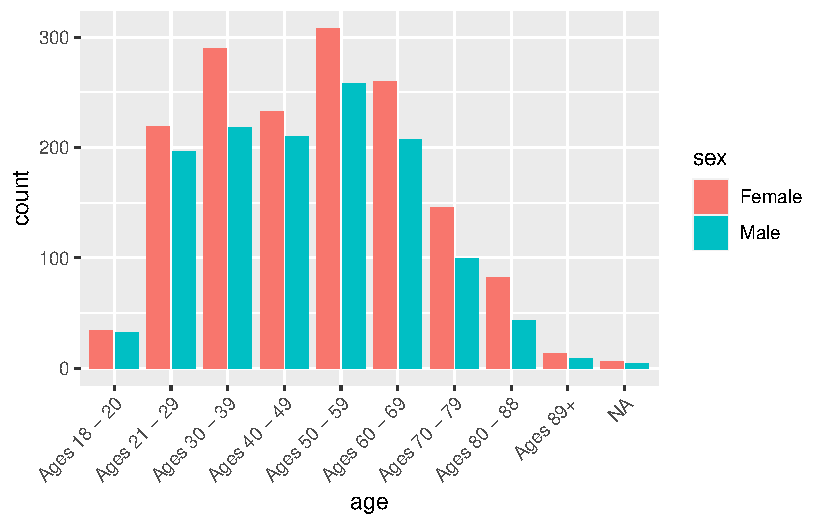
\includegraphics{paper_files/figure-pdf/fig-agesidebyside-1.pdf}

}

}

\subcaption{\label{fig-agesidebyside-1}Relationship between Age and Sex}
\end{minipage}%
%
\begin{minipage}[t]{0.50\linewidth}

{\centering 

\raisebox{-\height}{

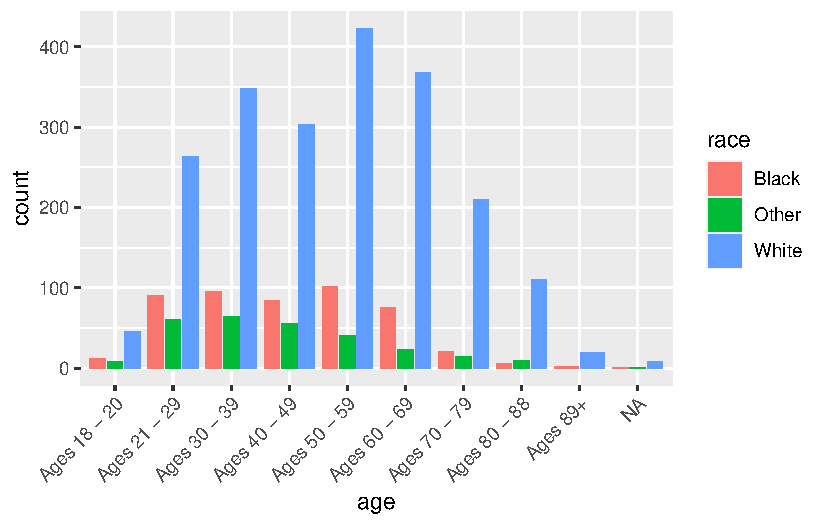
\includegraphics{paper_files/figure-pdf/fig-agesidebyside-2.pdf}

}

}

\subcaption{\label{fig-agesidebyside-2}Relationship Between Age and
Race}
\end{minipage}%

\caption{\label{fig-agesidebyside}Relationship between Age and Sex and
Age and Race}

\end{figure}

Most of the respondents of the 2016 GSS are adults ranging from ages 21
to 69 years old. The size of each age group between that range
oscillates within the right skewed distribution. The largest age group
respondent size is 50 to 59 years old. By graphing the variables, age
and sex in Figure~\ref{fig-agesidebyside}, we observe that there are
more female adults in each age group participating in this survey than
there are male adults. The overall distribution is skewed to the right.
The visualization of age and race in Figure~\ref{fig-agesidebyside}
demonstrates that the respondents that identify with the White racial
group comprises most of the respondent sample. This racial group is also
shown to have a near-symmetrical distribution. Conversely, the other
racial groups in this survey, Black and Other, are significantly the
minority of the survey sample. The Black and Other racial groups are
skewed to the right, illustrating that there are less individuals that
identify with these racial groups in the older age groups. According to
the 2020 US Census surveys, the most common racial group in America is
White or Caucasian, which means that the 2016 GSS data on this group
provides a relatively accurate representation of American society
(Jensen 2022).

\begin{figure}

{\centering 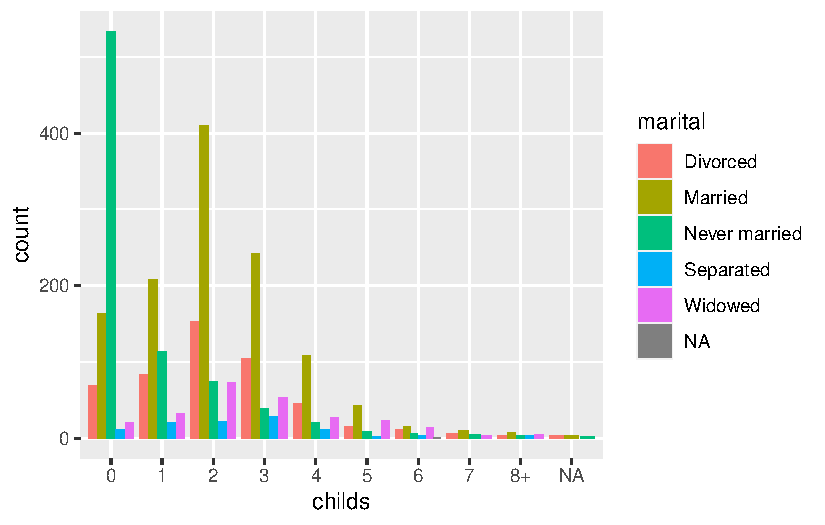
\includegraphics{paper_files/figure-pdf/fig-childsandmarital-1.pdf}

}

\caption{\label{fig-childsandmarital}Relationship between Marital Status
and Number of Children}

\end{figure}

According to Figure~\ref{fig-childsandmarital}, respondents who are
married have a right skew distribution of the number of children they
have, where the mode of the data is having two children. As for
individuals that responded as never having been married, the
distribution was exponential, in which the mode of this distribution is
having zero children. As the number of children increases, the number of
individuals who have never been married decreases. The distribution of
the other minority marital groups are skewed to the right. Overall, most
survey respondents have zero children.

\begin{figure}

{\centering 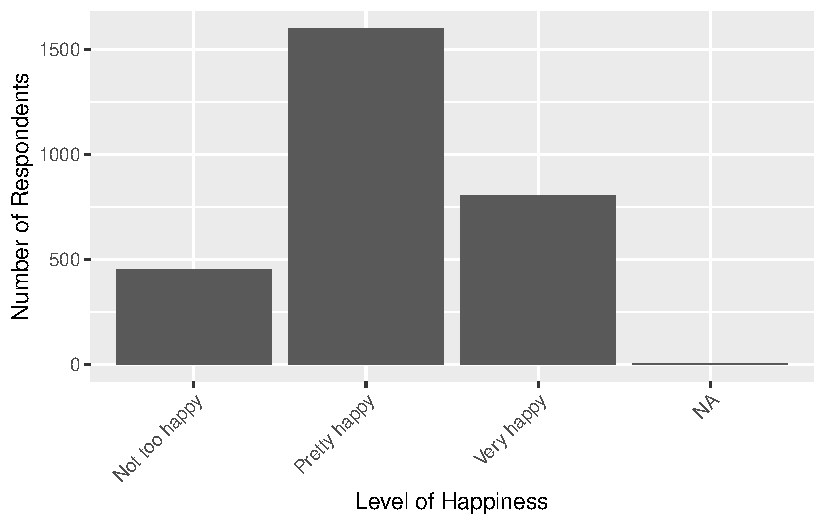
\includegraphics{paper_files/figure-pdf/fig-happiness-1.pdf}

}

\caption{\label{fig-happiness}Happiness Level Responses from Survey
Respondents}

\end{figure}

Figure~\ref{fig-happiness} demonstrates general happiness trends and
exhibits a left skew distribution. This illustrates that a significant
proportion of the respondents indicate that they are fairly happy and an
adequate proportion indicate that they are very happy. With a limited
number of options to measure happiness quantitatively, it is difficult
to discern a distribution on varying levels of happiness.

\hypertarget{results}{%
\section{Results}\label{results}}

\begin{figure}

{\centering 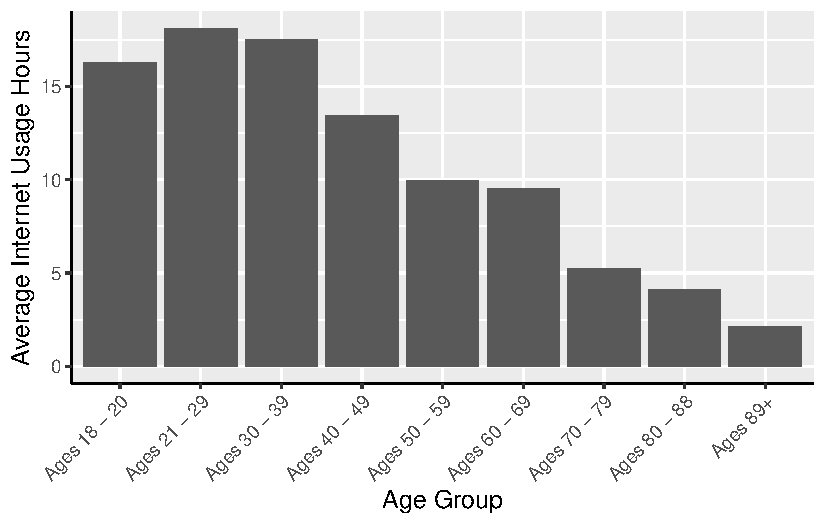
\includegraphics{paper_files/figure-pdf/fig-ageandinternet-1.pdf}

}

\caption{\label{fig-ageandinternet}Average Weekly Total of Internet Use
by Age Group}

\end{figure}

Figure~\ref{fig-ageandinternet} depicts the relationship between age and
average weekly Internet usage. The data on Internet usage hours for
various age groups are averaged to reduce any bias due to selectively
chosen survey responses. The curve on the graph is skewed to the right,
with its peak occurring in the 21 to 29 age group, which has the highest
Internet usage of approximately 18 hours per week. Subsequently,
Internet usage gradually declines with age, with the lowest usage
recorded in the 89+ age group at an average of 2 hours per week. This
graph indicates that young adults, particularly those aged 21 to 29,
spend more time on the Internet. As people age, their Internet usage
tends to decline gradually. The graph suggests a statistically
significant correlation between age and Internet usage, and the trend is
relatively clear.

\begin{figure}

{\centering 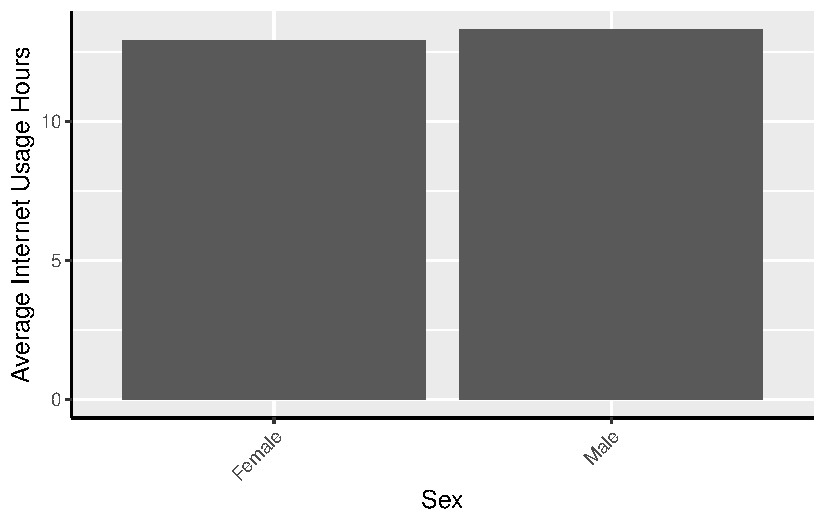
\includegraphics{paper_files/figure-pdf/fig-genderandinternet-1.pdf}

}

\caption{\label{fig-genderandinternet}Average Weekly Total of Internet
Use by Gender}

\end{figure}

Figure~\ref{fig-genderandinternet} illustrates the average weekly
Internet usage of two sexes. Similar to the age and Internet usage
graph, the data on Internet usage hours for different genders are
averaged to minimize any volunteering bias. The data shows that there is
no substantial difference between male and female Internet usage. Female
participants have an average of 12.9 hours per week spent on the
Internet, while male participants have a slightly higher average of 13.3
hours per week spent on the Internet. However, the gender selection in
this survey is limited, and further discussion regarding this limitation
can be found in the ethics and bias section Section~\ref{sec-bias}.

\begin{figure}

{\centering 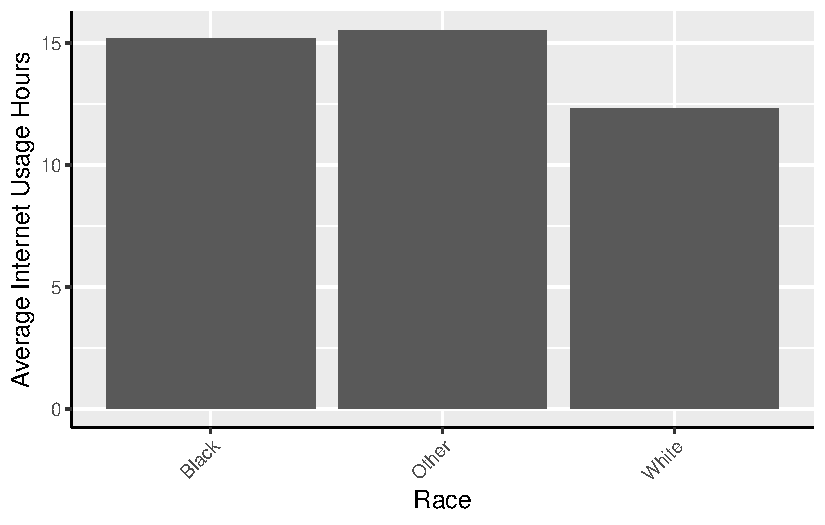
\includegraphics{paper_files/figure-pdf/fig-raceandinternet-1.pdf}

}

\caption{\label{fig-raceandinternet}Average Weekly Total of Internet Use
by Race}

\end{figure}

Figure~\ref{fig-raceandinternet} displays the average weekly Internet
usage of individuals belonging to different races. Based on the data, we
can observe that individuals who do not identify as either Black or
White have the highest Internet usage, with an average of 15.5 hours per
week. Black individuals have a similar level of Internet usage, also
averaging 15.2 hours per week. In contrast, White individuals tend to
have the lowest Internet usage, with an average of 12.3 hours per week.

\begin{figure}

{\centering 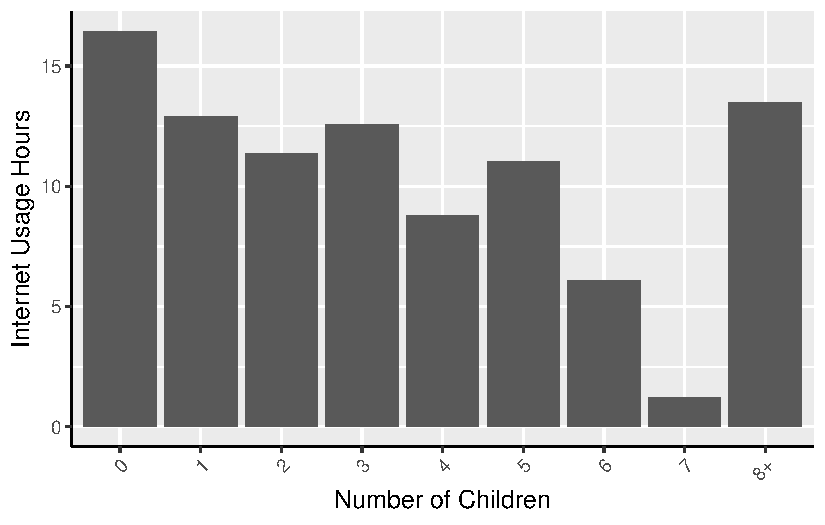
\includegraphics{paper_files/figure-pdf/fig-childrenandinternet-1.pdf}

}

\caption{\label{fig-childrenandinternet}Average Weekly Total of Internet
Use by Children}

\end{figure}

Figure~\ref{fig-childrenandinternet} shows the relationship between
respondents with a specific number of children and their weekly total
hours of Internet use. Respondents that do not have any children are the
group that uses the Internet the most during the week. Their average
amount of hours of weekly Internet use is approximately 16.5 hours. The
data demonstrates that there is an inverse relationship between the two
variables. This means that there is a gradual decrease of Internet use
hours as the number of children increases. The group that uses the least
amount of hours, with an average of approximately 1.5 hours of Internet
use weekly, are those with 7 children. However, the second largest group
that uses the Internet are those that reported having 8 children or
more, making this group an outlier.

\begin{figure}

{\centering 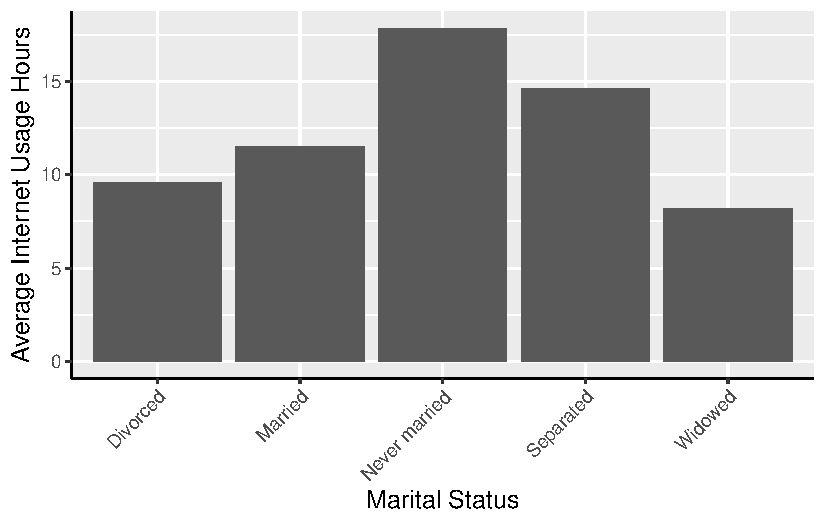
\includegraphics{paper_files/figure-pdf/fig-maritalandinternet-1.pdf}

}

\caption{\label{fig-maritalandinternet}Average Weekly Total of Internet
Use by Marital Status}

\end{figure}

Figure~\ref{fig-maritalandinternet} displays the relationship between
marital status and Internet usage in 2016. In accordance with popular
opinion, people who have never been married use the Internet the most,
with an average of around 17.5 hours per week. Most notably, people who
are widowed use the Internet the least, with an average of around 9.5
hours per week, perhaps due to the correlation between age and
widowhood. The graph suggests a significant difference in the Internet
use between these two population groups, with a difference of 8 hours
between the two.

\begin{figure}

{\centering 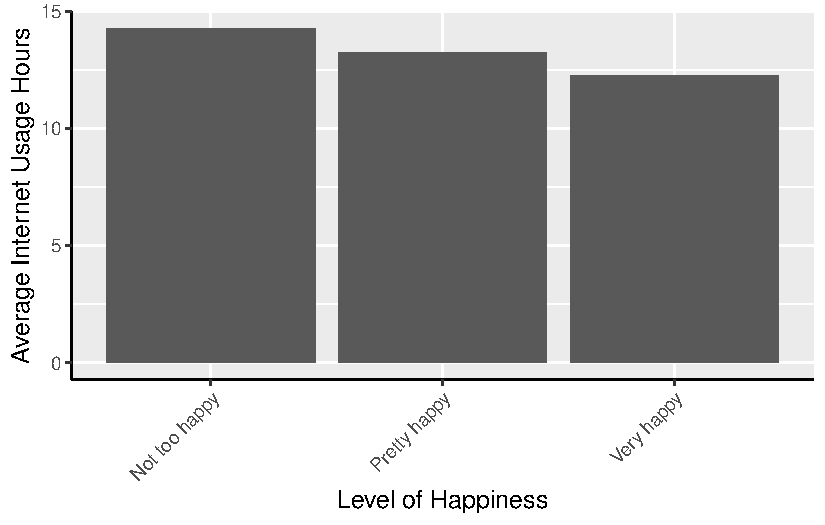
\includegraphics{paper_files/figure-pdf/fig-happyandinternet-1.pdf}

}

\caption{\label{fig-happyandinternet}Average Weekly Total of Internet
Use by Level of Happiness}

\end{figure}

Figure~\ref{fig-happyandinternet} displays the relationship between
perceived level of happiness and Internet usage in 2016. People who
reported the lowest level of happiness had the highest Internet usage,
with an average of around 14 hours per week. People who reported the
highest level of happiness had the lowest Internet usage, with an
average of around 12 hours per week. There seems to be a direct decrease
in Internet usage the more happy the respondent measures themselves to
be, with a difference of 2 hours between the happiest respondents and
least happy respondents.

\hypertarget{sec-discussion}{%
\section{Discussion}\label{sec-discussion}}

\hypertarget{sec-first-point}{%
\subsection{Aging Reduces the Amount of Hours Spent Using the
Internet}\label{sec-first-point}}

Based on the results, we find that as aging increases, the amount of
weekly total hour Internet use decreases. As shown in
Figure~\ref{fig-ageandinternet}, the majority of respondents that have
the highest number of weekly hours of Internet use are those between the
ages of 18 and 39 years old. The three age groups within this range have
the three largest Internet usages. By observing the tail of the
right-skewed distribution in Figure~\ref{fig-ageandinternet}, the graph
illustrates that as the age of respondents increases beginning from the
age range of 20-29 years old, the use of the Internet reduces. In this
era of developing technology and digital services, the Internet has
become a widely used source for information, commerce, communication,
and entertainment. According to our results, many young adults are
commonly online. This may be because they have the functional
capabilities of learning how to use the Internet and actually using the
Internet. Its ease and convenience allows users to have access to
instant information and communication, popularly used by young adults.
In comparison, those of older age tend to use the Internet less. The
reason for this may be because, as individuals age, they experience
declining changes in their physical, mental, and social abilities,
affecting their functional capacities. Research has shown that 23\% of
older adults indicate that having a physical or health condition makes
reading difficult or challenging (Smith 2019). This shows that those in
older age groups have barriers when it comes to using the Internet.
Although using the Internet is valuable to those of older age, as it
helps them connect with family members remotely and experience
socialization, the factors that make using the Internet challenging
keeps them from increasing their weekly use. Many older adults have
expressed that, when using technology and digital services, they would
need assistance (Smith 2019). Despite seniors being less likely than the
rest of the population to go online, once they understand how to use it,
it becomes a part of their everyday lives. Research has shown that 71\%
of seniors go online almost everyday and 11\% go online three to five
times weekly (Smith 2019). While many older adults understand the
beneficial aspect of the Internet, there still remains many non-users of
the Internet due to disabilities that come with aging (Smith 2019).

\hypertarget{sec-second-point}{%
\subsection{Marriage and Number of Children Reduces the Amount of Hours
Spent Using the Internet}\label{sec-second-point}}

\hypertarget{marital-status}{%
\subsubsection{Marital Status}\label{marital-status}}

As seen in Figure~\ref{fig-maritalandinternet}, people who have never
married use the Internet significantly more than those who are married
or who are widowed. This trend could partially be explained by the
correlation between age and being married, as those who have never been
married are more likely to be younger. In the United States in 2016, at
the time this survey data was collected, the median age of marriage was
28 years old for women and 30 years old for men ({``Median Age at First
Marriage (Women),''} n.d.). This statistic is consistent with the
findings of Figure~\ref{fig-ageandinternet}, which shows that Internet
usage is highest for people aged 21 to 29, people who are just prior to
the median age of marriage. This explanation is supported by the finding
that widowed people use the Internet the least, out of all of the
marital categories. Because widowhood is more likely in people who are
older, the correlation between age and Internet use is further reflected
here (Isherwood, King, and Luszcz 2017). Thus, the relationship between
marriage versus non-marriage and Internet use, in which those who have
never been married use the Internet more than those who are married, is
related to the inverse relationship between age and amount of average
Internet use stated in Section 4.1 above.

This trend of younger and non-married people using the Internet more
than older, married people could be further explained by the use of
online and digital dating apps by younger, non-married people as ways to
connect with people romantically. The United States is one of the
countries that uses online dating sites and apps the most, suggesting
that online dating is normalized in American culture and partially
explaining why younger, non-married people use the Internet much more
than their older, married counterparts (Buchholz 2023). The widespread
usage of handheld mobile devices that has become the norm for all age
groups, but especially younger people who are more likely to use social
media and online dating apps, furthers this.

A third contributing factor to this trend could be that non-married
individuals feel more isolated due to not meeting societal norms of
marriage and turn to the Internet to seek connections and community.
People who live in societies in which marriage is socially expected,
such as the United States, can feel isolated, for which using the
Internet can help them feel a sense of belonging that they find missing
in their lives (Himawan et al. 2021).

\hypertarget{number-of-children}{%
\subsubsection{Number of Children}\label{number-of-children}}

Figure~\ref{fig-childrenandinternet} demonstrates the relationship
between number of children of respondents and average weekly Internet
use. This graph shows that people with no children use the Internet more
than people who have children. Like Section 4.2.1 above, this could be
due to the correlation between age and having children: those who are
older are more likely to have children than those who are younger. The
median age at which women have children is 30 years of age, which is
consistent with the findings of Figure~\ref{fig-ageandinternet}, which
states that people in their 20s use the Internet the most (Morse 2022).
This general inverse relationship between number of children and
Internet use, is related to the inverse relationship between age and
amount of average Internet use stated in Section 4.1 above. The outlier
of the ``8+'' children category has a high Internet usage because there
were only 6 people who responded about their Internet usage in that
category (compared to the approximately 500 people who responded about
their Internet usage in the ``0'' children category), such that the
result was skewed by one participant who reported 60 hours of Internet
use.

This trend could also be explained by the amount of personal time that
people have for themselves. Personal use is one of the main activities
of Internet use (including instant messaging and social media), and
people with children are less likely to have time for themselves as they
spend time caring for their children (Petrosyan 2023). This likely
increases with more children. Thus, the relatively inverted relationship
between number of children and Internet use could be partially explained
by the inverted relationship between number of children and personal
time.

However, the Internet has increasingly come to be a key resource for
parenting, both for getting information and for receiving support
(Duggan et al. 2015). This explains why average Internet use is
relatively similar across people with 1 child to 5 children.

\hypertarget{sec-third-point}{%
\subsection{Happiness Reduces the Amount of Hours Spent Using the
Internet}\label{sec-third-point}}

In a previous study, we found a potential correlation between happiness
and Internet usage. Specifically, individuals who reported lower
Internet usage tended to have higher levels of happiness. There are a
few reasons that may contribute to this finding.

We suspect this finding may be attributed to various factors related to
social media usage, given that people spend an average of 2 hours and 31
minutes daily on social media (Georgiev 2023). Our secondary research
indicates that certain aspects of the Internet, such as social media,
can negatively impact psychological health. Excessive use of social
media can result in addiction, anxiety, depression, or isolation.
Furthermore, social media can become a substitute for real-life social
interaction, causing individuals to feel lonely and disconnected.
Comparing oneself unfavourably with Internet social figures can also
lead to low self-esteem and negative body image, while cyberbullying can
have potential mental health implications for individuals who spend long
hours on the Internet. A study by the University of Pennsylvania in 2018
found that reducing social media use to 30 minutes a day resulted in a
significant reduction in anxiety, depression, loneliness, and sleep
problems (Robinson and Smith 2023).

Additionally, research suggests that spending more time online can make
children less happy with their lives. For instance, a study by the
University of Sheffield concluded that spending an extra hour a day on
social networks reduces the probability of being completely happy with
life overall by approximately 14 percentage points (Sheffield 2017).
Thus, we have reason to believe that Internet usage, particularly social
media usage, can have a negative impact on happiness levels to some
extent and affect the relationship between happiness and Internet usage.

Another factor that could contribute to the correlation between
happiness and Internet usage is a fulfilling real life. Engaging in
offline activities, such as spending time with loved ones, pursuing
hobbies, or achieving personal goals, can be more rewarding than
spending time online. This can lead individuals to prioritize fulfilling
activities over aimless scrolling through the Internet and decrease
their need for validation or connection through social media and other
online platforms. Thus, individuals who are fulfilled in their offline
lives may have lower Internet usage hours and higher happiness levels.

\hypertarget{sec-weaknessesandnextsteps}{%
\subsection{Weaknesses and Next
Steps}\label{sec-weaknessesandnextsteps}}

\hypertarget{sec-weaknesses}{%
\subsubsection{Weakness}\label{sec-weaknesses}}

A key weakness in our analysis was that we removed non-responses from
our data, which may have made our data for Internet use not as accurate
in reflecting what the actual population's Internet use looks like. A
central reason as to why participant's may have chosen not to respond to
the question about Internet use could be embarrassment: admitting that
one spends too much time on the Internet could be embarrassing, so those
who have higher Internet usage are more likely not to respond to this
question. This is a very real concern as Internet addiction is emerging
rapidly in our increasingly digital world, and several countries have
even identified it as a public health concern (Cash et al. 2012).

Another weakness in our analysis is the self-reported nature of the
results, meaning there was some bias in questions with ambiguous word
choice, such as our happiness variable. The definition of the different
response options to the happiness variable survey question of ``not so
happy'', ``fairly happy'', and ``very happy'' will vary depending on the
individual, as well as the day or time of day. Thus, our analysis of the
relationship between happiness and Internet use may be biased.

\hypertarget{next-steps}{%
\subsubsection{Next Steps}\label{next-steps}}

To address our second identified weakness in
Section~\ref{sec-weaknesses} above, implementing a supplementary survey
with more detailed questions, particularly about race and gender (as
mentioned in Section~\ref{sec-questionnaire}) and more straightforward
question answers (e.g.~a number scale for happiness variable) would
allow for more in-depth analysis.

In addition, conducting further research on the different uses of the
Internet based on population groups would be a reasonable next step, now
that we have determined which population groups use the Internet the
most and the least.

Finally, looking at how COVID-19 impacted Internet usage would be a
particularly interesting avenue of research to pursue, especially with
the increase in online activities (e.g.~work from home, online classes,
widespread use of Zoom, etc.). It would be interesting to compare our
analysis of American population groups that used the Internet the most
in 2016, with 2020 (during the COVID-19 pandemic) and with 2022
(post-COVID-19 pandemic).

\hypertarget{sec-bias}{%
\subsection{Ethics and Bias}\label{sec-bias}}

Based on the data collection methodology provided by GSS, we have
identified some potential biases that could arise. The survey's target
population consists of adults aged 18 and above who reside in households
in the United States. Since this sampling approach focuses only on a
specific age group, our analysis may be biased with respect to the age
factor. GSS also claimed to be strictly voluntary. While this approach
supports research ethics by respecting individuals' autonomy and right
to privacy, it can also result in volunteer bias. The GSS sample is from
a combination of urban, suburban, and rural geographic areas, but only a
few thousand respondents are interviewed in the main study. The small
sample size may lead to chance findings. We also suspect potential
sampling bias may affect our end results. However, with not enough
information disclosed, we are unable to confirm that. The gender and
race options provided by the GSS survey are limited. Participants are
only given the options of selecting either ``Female'' or ``Male'' for
gender, and ``Black,'' ``White,'' or ``Other'' for race. This narrow
selection does not provide an adequate range of options for survey
participants.

\hypertarget{appendix}{%
\section{Appendix}\label{appendix}}

\hypertarget{references}{%
\section*{References}\label{references}}
\addcontentsline{toc}{section}{References}

\hypertarget{refs}{}
\begin{CSLReferences}{1}{0}
\leavevmode\vadjust pre{\hypertarget{ref-citem1}{}}%
{``A Short History of the Internet.''} 2020. National Science; Media
Museum.
\url{https://www.scienceandmediamuseum.org.uk/objects-and-stories/short-history-internet\#:~:text=Consequently\%2C\%20the\%20number\%20of\%20websites,around\%2010\%20million\%20global\%20users}.

\leavevmode\vadjust pre{\hypertarget{ref-cite3}{}}%
{``About the GSS.''} n.d. NORC.
\url{https://gss.norc.org/About-The-GSS}.

\leavevmode\vadjust pre{\hypertarget{ref-cite15}{}}%
Alexander, Rohan. 2023. {``Telling Stories with Data.''}
\url{https://tellingstorieswithdata.com/06-farm.html\#measurement}.

\leavevmode\vadjust pre{\hypertarget{ref-cite21}{}}%
Buchholz, Katharina. 2023. {``How the World Dates Online.''}
\emph{Statista}.
\url{https://www.statista.com/chart/24165/online-dating-penetration-rate-revenue-selected-countries/\#:~:text=The\%20United\%20States\%20is\%20the,of\%20\%242.5\%20billion\%20in\%202023.}

\leavevmode\vadjust pre{\hypertarget{ref-cite14}{}}%
Bureau, US Census. 2022. {``About the Topic of Race.''}
\url{https://www.census.gov/topics/population/race/about.html}.

\leavevmode\vadjust pre{\hypertarget{ref-cite26}{}}%
Cash, Hilarie, Cosette D Rae, Ann H Steel, and Alexander Winkler. 2012.
{``Internet Addiction: A Brief Summary of Research and Practice.''}
\emph{Current Psychiatry Reviews}.
\url{https://www.ncbi.nlm.nih.gov/pmc/articles/PMC3480687/}.

\leavevmode\vadjust pre{\hypertarget{ref-cite25}{}}%
Duggan, Maeve, Amanda Lenhart, Cliff Lampe, and Nicole B. Elisson. 2015.
{``Parents and Social Media.''} Pew Research Center.
\url{https://www.pewresearch.org/internet/2015/07/16/parents-and-social-media/}.

\leavevmode\vadjust pre{\hypertarget{ref-cite13}{}}%
{``For Survey Participants.''} n.d. NORC.
\url{https://gss.norc.org/For-Survey-Participants}.

\leavevmode\vadjust pre{\hypertarget{ref-cite5}{}}%
{``Frequently Asked Questions.''} n.d. NORC.
\url{https://gss.norc.org/faq}.

\leavevmode\vadjust pre{\hypertarget{ref-citea1}{}}%
Georgiev, Deyan. 2023. {``How Much Time Do People Spend on Social Media
in 2023?''} Techjury.
\url{https://techjury.net/blog/time-spent-on-social-media/\#gref}.

\leavevmode\vadjust pre{\hypertarget{ref-lessR}{}}%
Gerbing, David W. 2021. {``Enhancement of the Command-Line Environment
for Use in the Introductory Statistics Course and Beyond.''}
\emph{Journal of Statistics and Data Science Education} 29 (3): 251--56.
\url{https://doi.org/10.1080/26939169.2021.1999871}.

\leavevmode\vadjust pre{\hypertarget{ref-cite6}{}}%
{``GSS 1972-2018 Cross-Section Codebook: Appendix a - Sampling Design
and Weighting.''} n.d. \url{https://gss.norc.org/Get-Documentation}.

\leavevmode\vadjust pre{\hypertarget{ref-gss}{}}%
{``GSS Data Explorer: NORC at the University of Chicago.''} n.d. NORC.
\url{https://gssdataexplorer.norc.org/}.

\leavevmode\vadjust pre{\hypertarget{ref-cite22}{}}%
Himawan, Karel Karsten, Mair Underwood, Matthew Bambling, and Sisira
Edirippulige. 2021. {``Being Single When Marriage Is the Norm: Internet
Use and the Well-Being of Never-Married Adults in Indonesia - Current
Psychology.''} \emph{Current Psychology}. Springer US.
\url{https://link.springer.com/article/10.1007/s12144-021-01367-6}.

\leavevmode\vadjust pre{\hypertarget{ref-cite20}{}}%
Isherwood, L. M., D. S. King, and M. A. Luszcz. 2017. {``Widowhood in
the Fourth Age: Support Exchange, Relationships and Social
Participation: Ageing \&Amp; Society.''} \emph{Ageing \& Society}.
Cambridge University Press.
\url{https://www.cambridge.org/core/journals/ageing-and-society/article/abs/widowhood-in-the-fourth-age-support-exchange-relationships-and-social-participation/357209AB1A6F356266FEEA0B7B604A9D}.

\leavevmode\vadjust pre{\hypertarget{ref-citem3}{}}%
Jensen, Eric. 2022. {``The Chance That Two People Chosen at Random Are
of Different Race or Ethnicity Groups Has Increased Since 2010.''} US
Census.
\url{https://www.census.gov/library/stories/2021/08/2020-united-states-population-more-racially-ethnically-diverse-than-2010.html}.

\leavevmode\vadjust pre{\hypertarget{ref-cite4}{}}%
{``Key Trends.''} n.d. \emph{NORC}.
\url{https://gssdataexplorer.norc.org/trends}.

\leavevmode\vadjust pre{\hypertarget{ref-citem2}{}}%
Lane, Anna Beth. 2022. {``14 Ways the Internet Improves Our Lives.''}
Community Tech Network.
\url{https://communitytechnetwork.org/blog/14-ways-the-internet-improves-our-lives/\#:~:text=Not\%20only\%20is\%20access\%20to,with\%20large\%20numbers\%20of\%20people}.

\leavevmode\vadjust pre{\hypertarget{ref-cite19}{}}%
{``Median Age at First Marriage (Women).''} n.d. Population Reference
Bureau.
\url{https://www.prb.org/usdata/indicator/marriage-age-women/snapshot/}.

\leavevmode\vadjust pre{\hypertarget{ref-cite23}{}}%
Morse, Anne. 2022. {``Stable Fertility Rates 1990-2019 Mask Distinct
Variations by Age.''} US Census Bureau.
\url{https://www.census.gov/library/stories/2022/04/fertility-rates-declined-for-younger-women-increased-for-older-women.html}.

\leavevmode\vadjust pre{\hypertarget{ref-here}{}}%
Müller, Kirill. 2020. \emph{Here: A Simpler Way to Find Your Files}.
\url{https://CRAN.R-project.org/package=here}.

\leavevmode\vadjust pre{\hypertarget{ref-cite24}{}}%
Petrosyan, Ani. 2023. {``Internet Activities of u.s. Users 2021.''}
\emph{Statista}.
\url{https://www.statista.com/statistics/183910/internet-activities-of-us-users/\#:~:text=As\%20of\%20November\%202021\%2C\%20it,the\%20country\%20used\%20messaging\%20services.}

\leavevmode\vadjust pre{\hypertarget{ref-R}{}}%
R Core Team. 2020. \emph{R: A Language and Environment for Statistical
Computing}. Vienna, Austria: R Foundation for Statistical Computing.
\url{https://www.R-project.org/}.

\leavevmode\vadjust pre{\hypertarget{ref-citea2}{}}%
Robinson, Lawrence, and Melinda Smith. 2023. {``Social Media and Mental
Health.''} HelpGuide.org.
\url{https://www.helpguide.org/articles/mental-health/social-media-and-mental-health.htm\#:~:text=A\%202018\%20University\%20of\%20Pennsylvania,to\%20improve\%20your\%20mental\%20health}.

\leavevmode\vadjust pre{\hypertarget{ref-citea3}{}}%
Sheffield, University of. 2017. {``More Time Spent Online Makes Children
Less Happy with Their Lives, Research Finds.''} \emph{More Time Spent
Online Makes Children Less Happy with Their Lives, Research Finds -
Archive - News Archive - The University of Sheffield}.
\url{https://www.sheffield.ac.uk/news/nr/social-media-economics-research-happiness-1.694959}.

\leavevmode\vadjust pre{\hypertarget{ref-citem4}{}}%
Smith, Aaron. 2019. {``Attitudes, Impacts, and Barriers to Adoption.''}
Pew Research Center.
\url{https://www.pewresearch.org/internet/2014/04/03/attitudes-impacts-and-barriers-to-adoption/}.

\leavevmode\vadjust pre{\hypertarget{ref-reshape2}{}}%
Wickham, Hadley. 2007. {``Reshaping Data with the {reshape} Package.''}
\emph{Journal of Statistical Software} 21 (12): 1--20.
\url{http://www.jstatsoft.org/v21/i12/}.

\leavevmode\vadjust pre{\hypertarget{ref-ggplot2}{}}%
---------. 2016. \emph{Ggplot2: Elegant Graphics for Data Analysis}.
Springer-Verlag New York. \url{https://ggplot2.tidyverse.org}.

\leavevmode\vadjust pre{\hypertarget{ref-tidyverse}{}}%
Wickham, Hadley, Mara Averick, Jennifer Bryan, Winston Chang, Lucy
D'Agostino McGowan, Romain François, Garrett Grolemund, et al. 2019.
{``Welcome to the {tidyverse}.''} \emph{Journal of Open Source Software}
4 (43): 1686. \url{https://doi.org/10.21105/joss.01686}.

\leavevmode\vadjust pre{\hypertarget{ref-haven}{}}%
Wickham, Hadley, Evan Miller, and Danny Smith. 2022. \emph{Haven: Import
and Export 'SPSS', 'Stata' and 'SAS' Files}.
\url{https://CRAN.R-project.org/package=haven}.

\leavevmode\vadjust pre{\hypertarget{ref-tidyr}{}}%
Wickham, Hadley, Davis Vaughan, and Maximilian Girlich. 2023.
\emph{Tidyr: Tidy Messy Data}.
\url{https://CRAN.R-project.org/package=tidyr}.

\leavevmode\vadjust pre{\hypertarget{ref-knitr}{}}%
Xie, Yihui. 2023. \emph{Knitr: A General-Purpose Package for Dynamic
Report Generation in r}. \url{https://yihui.org/knitr/}.

\leavevmode\vadjust pre{\hypertarget{ref-kableExtra}{}}%
Zhu, Hao. 2021. \emph{kableExtra: Construct Complex Table with 'Kable'
and Pipe Syntax}. \url{https://CRAN.R-project.org/package=kableExtra}.

\end{CSLReferences}



\end{document}
